\documentclass{article}
\usepackage{graphicx} % Required for inserting images
\usepackage[nonumberlist]{glossaries}
\usepackage[italian]{babel}
\usepackage{hyperref}
\usepackage[noabbrev]{cleveref}
\usepackage[margin=1in]{geometry}
\usepackage{biblatex}

\usepackage{bera}% optional: just to have a nice mono-spaced font
\usepackage{listings}
\usepackage{xcolor}

\colorlet{punct}{red!60!black}
\definecolor{background}{HTML}{EEEEEE}
\definecolor{delim}{RGB}{20,105,176}
\colorlet{numb}{magenta!60!black}

\lstdefinelanguage{json}{
    basicstyle=\normalfont\ttfamily,
    numbers=left,
    numberstyle=\scriptsize,
    stepnumber=1,
    numbersep=8pt,
    showstringspaces=false,
    breaklines=true,
    frame=lines,
    backgroundcolor=\color{background},
    literate=
     *{0}{{{\color{numb}0}}}{1}
      {1}{{{\color{numb}1}}}{1}
      {2}{{{\color{numb}2}}}{1}
      {3}{{{\color{numb}3}}}{1}
      {4}{{{\color{numb}4}}}{1}
      {5}{{{\color{numb}5}}}{1}
      {6}{{{\color{numb}6}}}{1}
      {7}{{{\color{numb}7}}}{1}
      {8}{{{\color{numb}8}}}{1}
      {9}{{{\color{numb}9}}}{1}
      {:}{{{\color{punct}{:}}}}{1}
      {,}{{{\color{punct}{,}}}}{1}
      {\{}{{{\color{delim}{\{}}}}{1}
      {\}}{{{\color{delim}{\}}}}}{1}
      {[}{{{\color{delim}{[}}}}{1}
      {]}{{{\color{delim}{]}}}}{1},
}

\usepackage{forest}

\definecolor{folderbg}{RGB}{124,166,198}
\definecolor{folderborder}{RGB}{110,144,169}

\def\Size{4pt}
\tikzset{
      folder/.pic={
        \filldraw[draw=folderborder,top color=folderbg!50,bottom color=folderbg]
          (-1.05*\Size,0.2\Size+5pt) rectangle ++(.75*\Size,-0.2\Size-5pt);  
        \filldraw[draw=folderborder,top color=folderbg!50,bottom color=folderbg]
          (-1.15*\Size,-\Size) rectangle (1.15*\Size,\Size);
      }
    }

\crefformat{section}{\S#2#1#3}
\crefformat{subsection}{\S#2#1#3}
\crefformat{subsubsection}{\S#2#1#3}
\crefformat{figure}{#2Figura~#1#3}
\crefformat{footnote}{#2\footnotemark[#1]#3}
\crefformat{table}{#2Tabella~#1#3}
\crefformat{equation}{#2Equazione~#1#3}
\crefformat{chapter}{#2Capitolo~#1#3}

\addbibresource{refs.bib}

\renewcommand{\contentsname}{Indice}

\makeglossaries

\newglossaryentry{player} 
{  
    name={player (\textmd{oppure} giocatore)},
    text=giocatore,
    description=è l'entità che può eseguire un turno nei round di un game. Un player può essere umano o un robot
}

\newglossaryentry{game}
{
    name={game (\textmd{oppure} gioco, partita)},
    text=partita,
    description={è l'entità principale del sistema. Un game è composto da più round}
}

\newglossaryentry{round}
{
    name=round,
    text=round,
    description={è l'entità che contiene le informazioni di gioco principali. Ogni game è composto da un numero 
    finito di round durante il quale ciascun giocatore effettua la propria giocata}
}

\newglossaryentry{turn}
{
    name={turn (\textmd{oppure} turno)},
    text=turno,
    description={è l'unità indivisibile di un round e rappresenta le azioni di un giocatore durante il round. Quindi contiene informazioni sull'esito dell'esecuzione dei test ed i relativi 
    risultati nonché le classi generate per risolvere il problema}
}

\begin{document}

\begin{titlepage}
    \begin{center}
        \vspace*{1cm}
            
        \Huge
        \textbf{Software Architecture Design}
            
        \vspace{0.5cm}
        \LARGE
        Game Repository - Iterazione 3
        
        \vfill
        \vspace{0.8cm}
        
        \Large
        Angelino Pasquale - M63001481 \\
        Capasso Giuseppe -  M63001498 \\
        Dinetti Andrea -  M63001496

    \end{center}
\end{titlepage}

\thispagestyle{empty}

\printglossaries

\newpage
\thispagestyle{empty}
\tableofcontents

\newpage
\thispagestyle{empty}
\section*{Introduzione}
In questa sezione, sarà effettuata una breve descrizione del progetto focalizzandosi sul \textit{task} assegnato.\\ 

L'attività assegnata prevede la progettazione e implementazione del componente \textit{Game Repository} che si occupa di memorizzare, per ogni \gls{game} giocata, informazioni quali il tipo, i \gls{round} giocati, le classi di test prodotte dai giocatori.

Il gruppo si coordina e gestisce le proprie attività con questo progetto
(consultabile al seguente \href{https://github.com/users/alarmfox/projects/2}{link}) in linea con le metodologie di sviluppo AGILE.

\newpage
\section{Analisi delle \textit{review} e iterazioni precedenti}
A valle delle precedenti iterazioni, è stato aggiunto il requisito di gestione dei punteggi generati dai robot (\textit{randoop} e \textit{evosuite}). Infatti, secondo la nuova architettura questi dati saranno pre generati all'atto del caricamento di una classe dall'amministratore.
Il nuovo requisito è stato integrato nel diagramma E/R utilizzato per modellare il dominio di applicazione in \cref{fig:er}.

\begin{figure}
    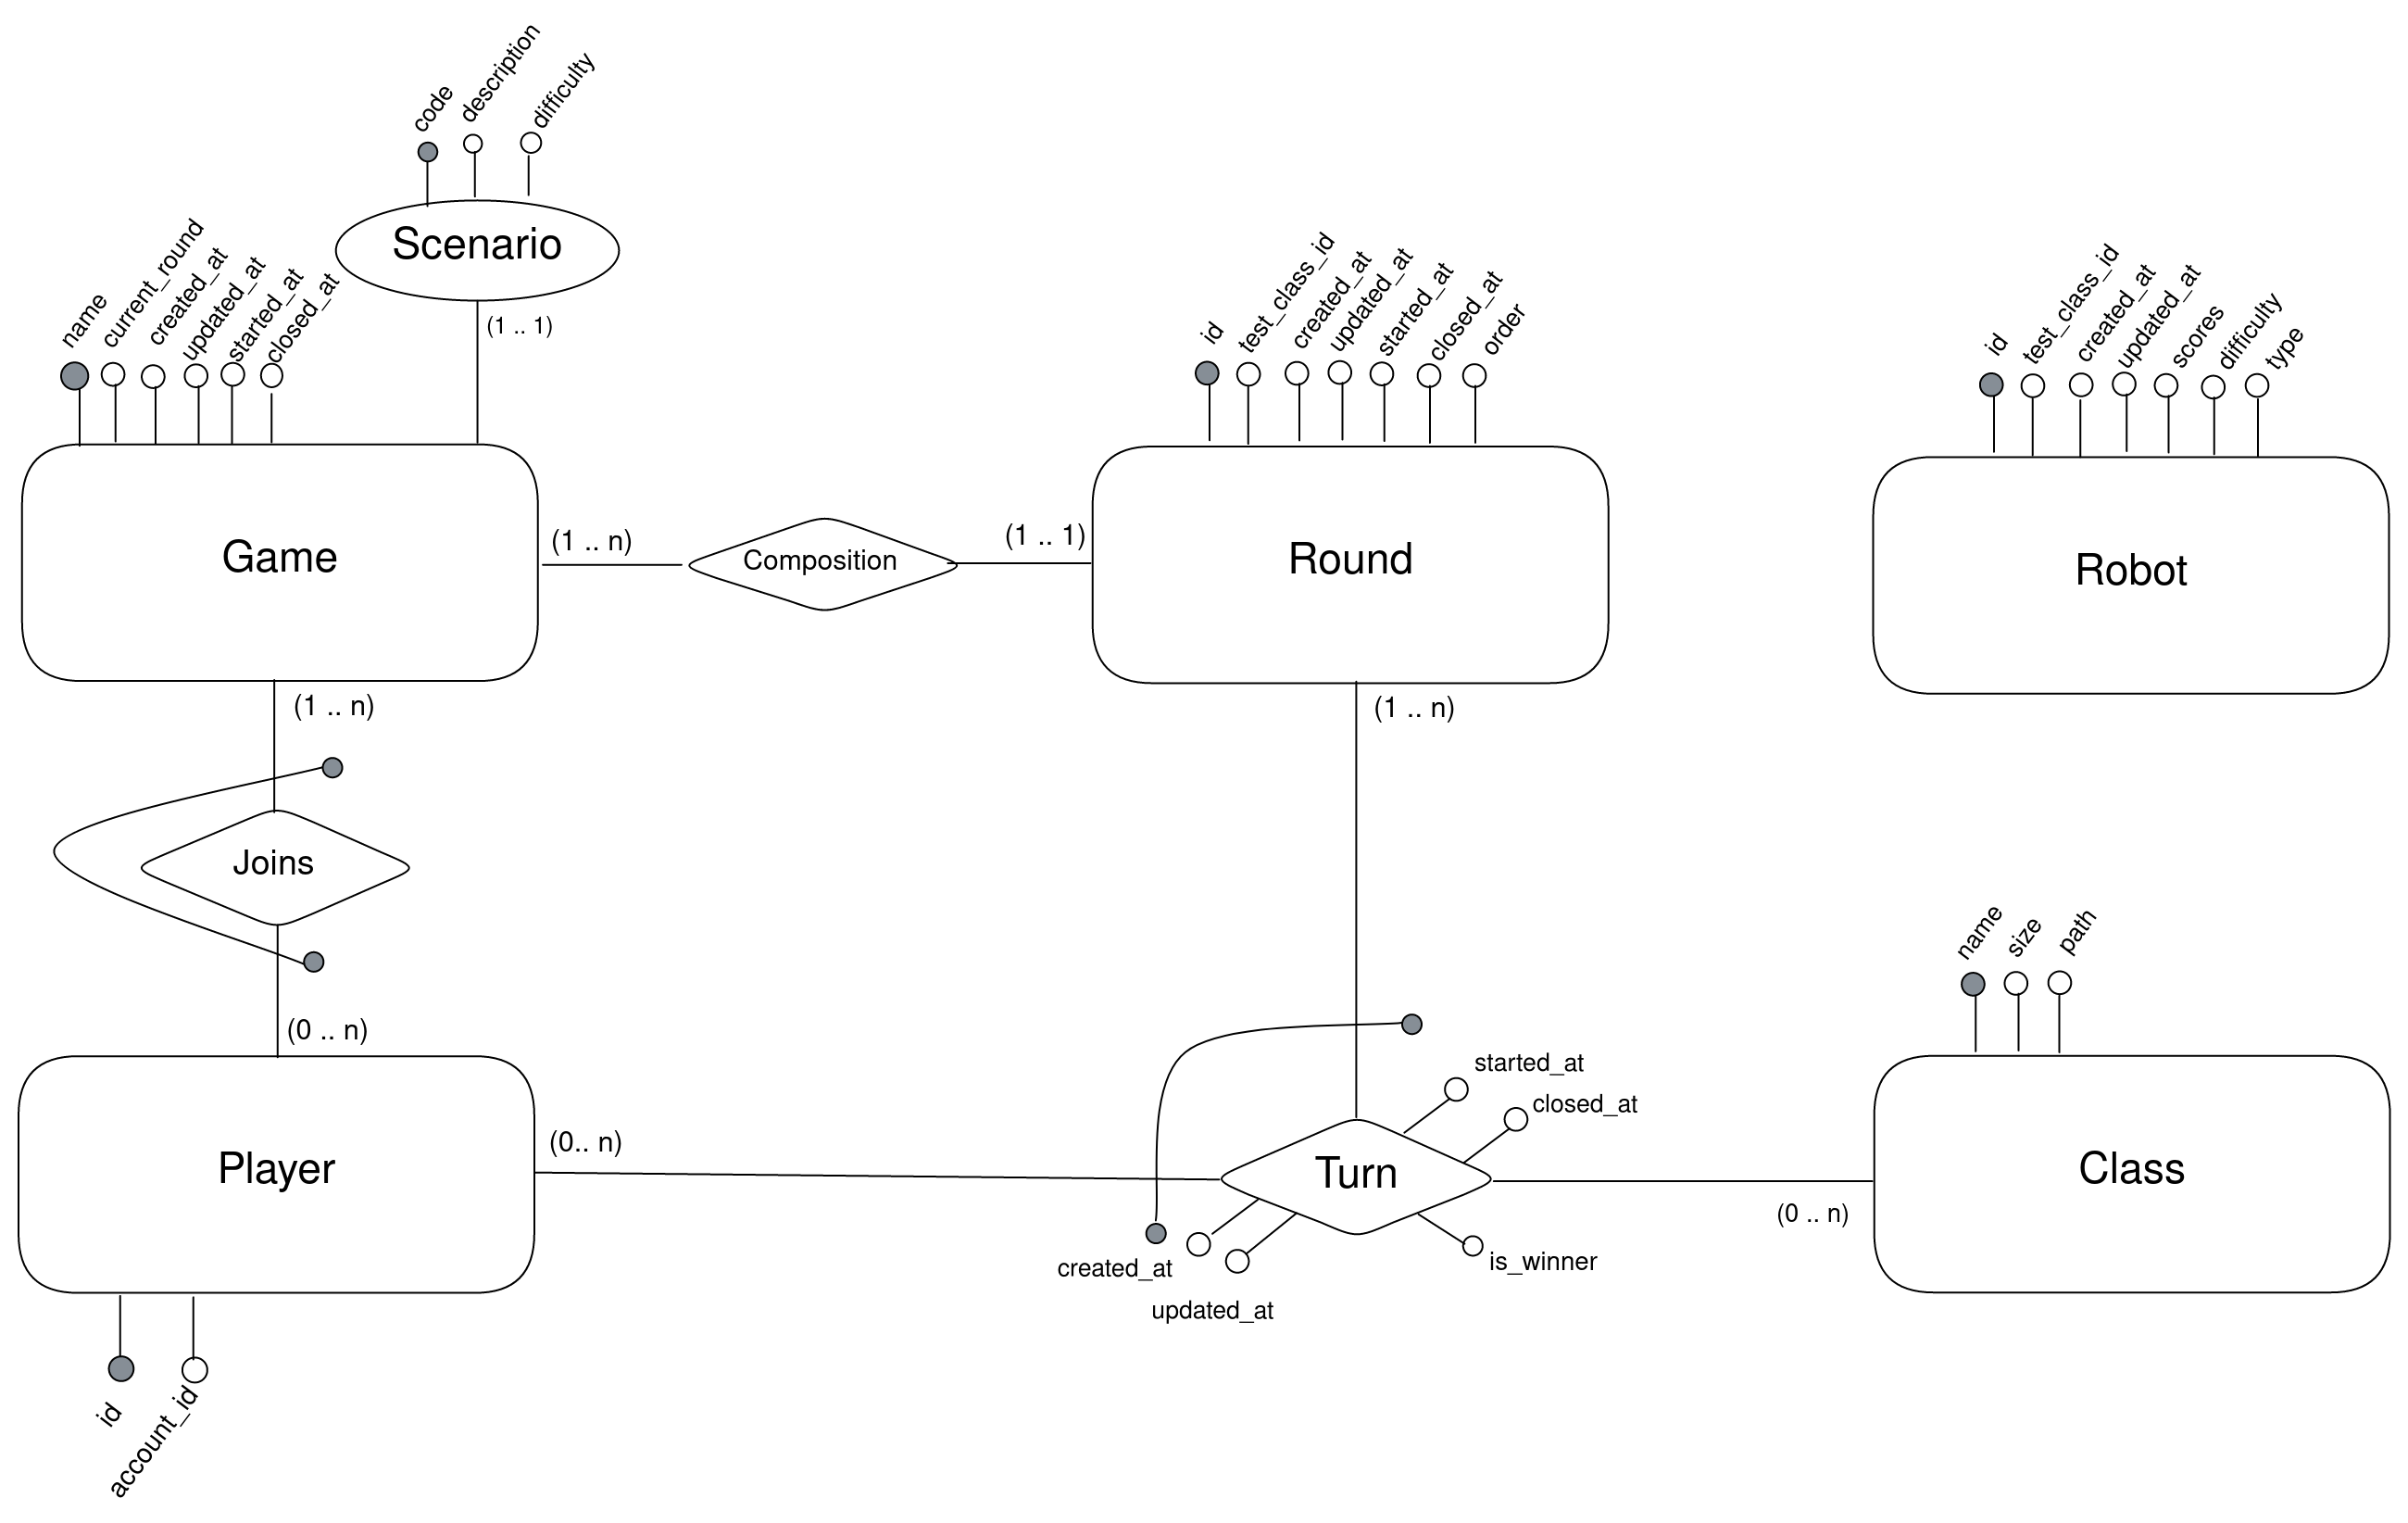
\includegraphics[width=\textwidth]{images/er.png}
    \caption{Modello E/R}
    \label{fig:er}
\end{figure}

Inoltre, l'architettura della soluzione è stata modificata come mostrato in \cref{fig:arch}.
\begin{figure}
    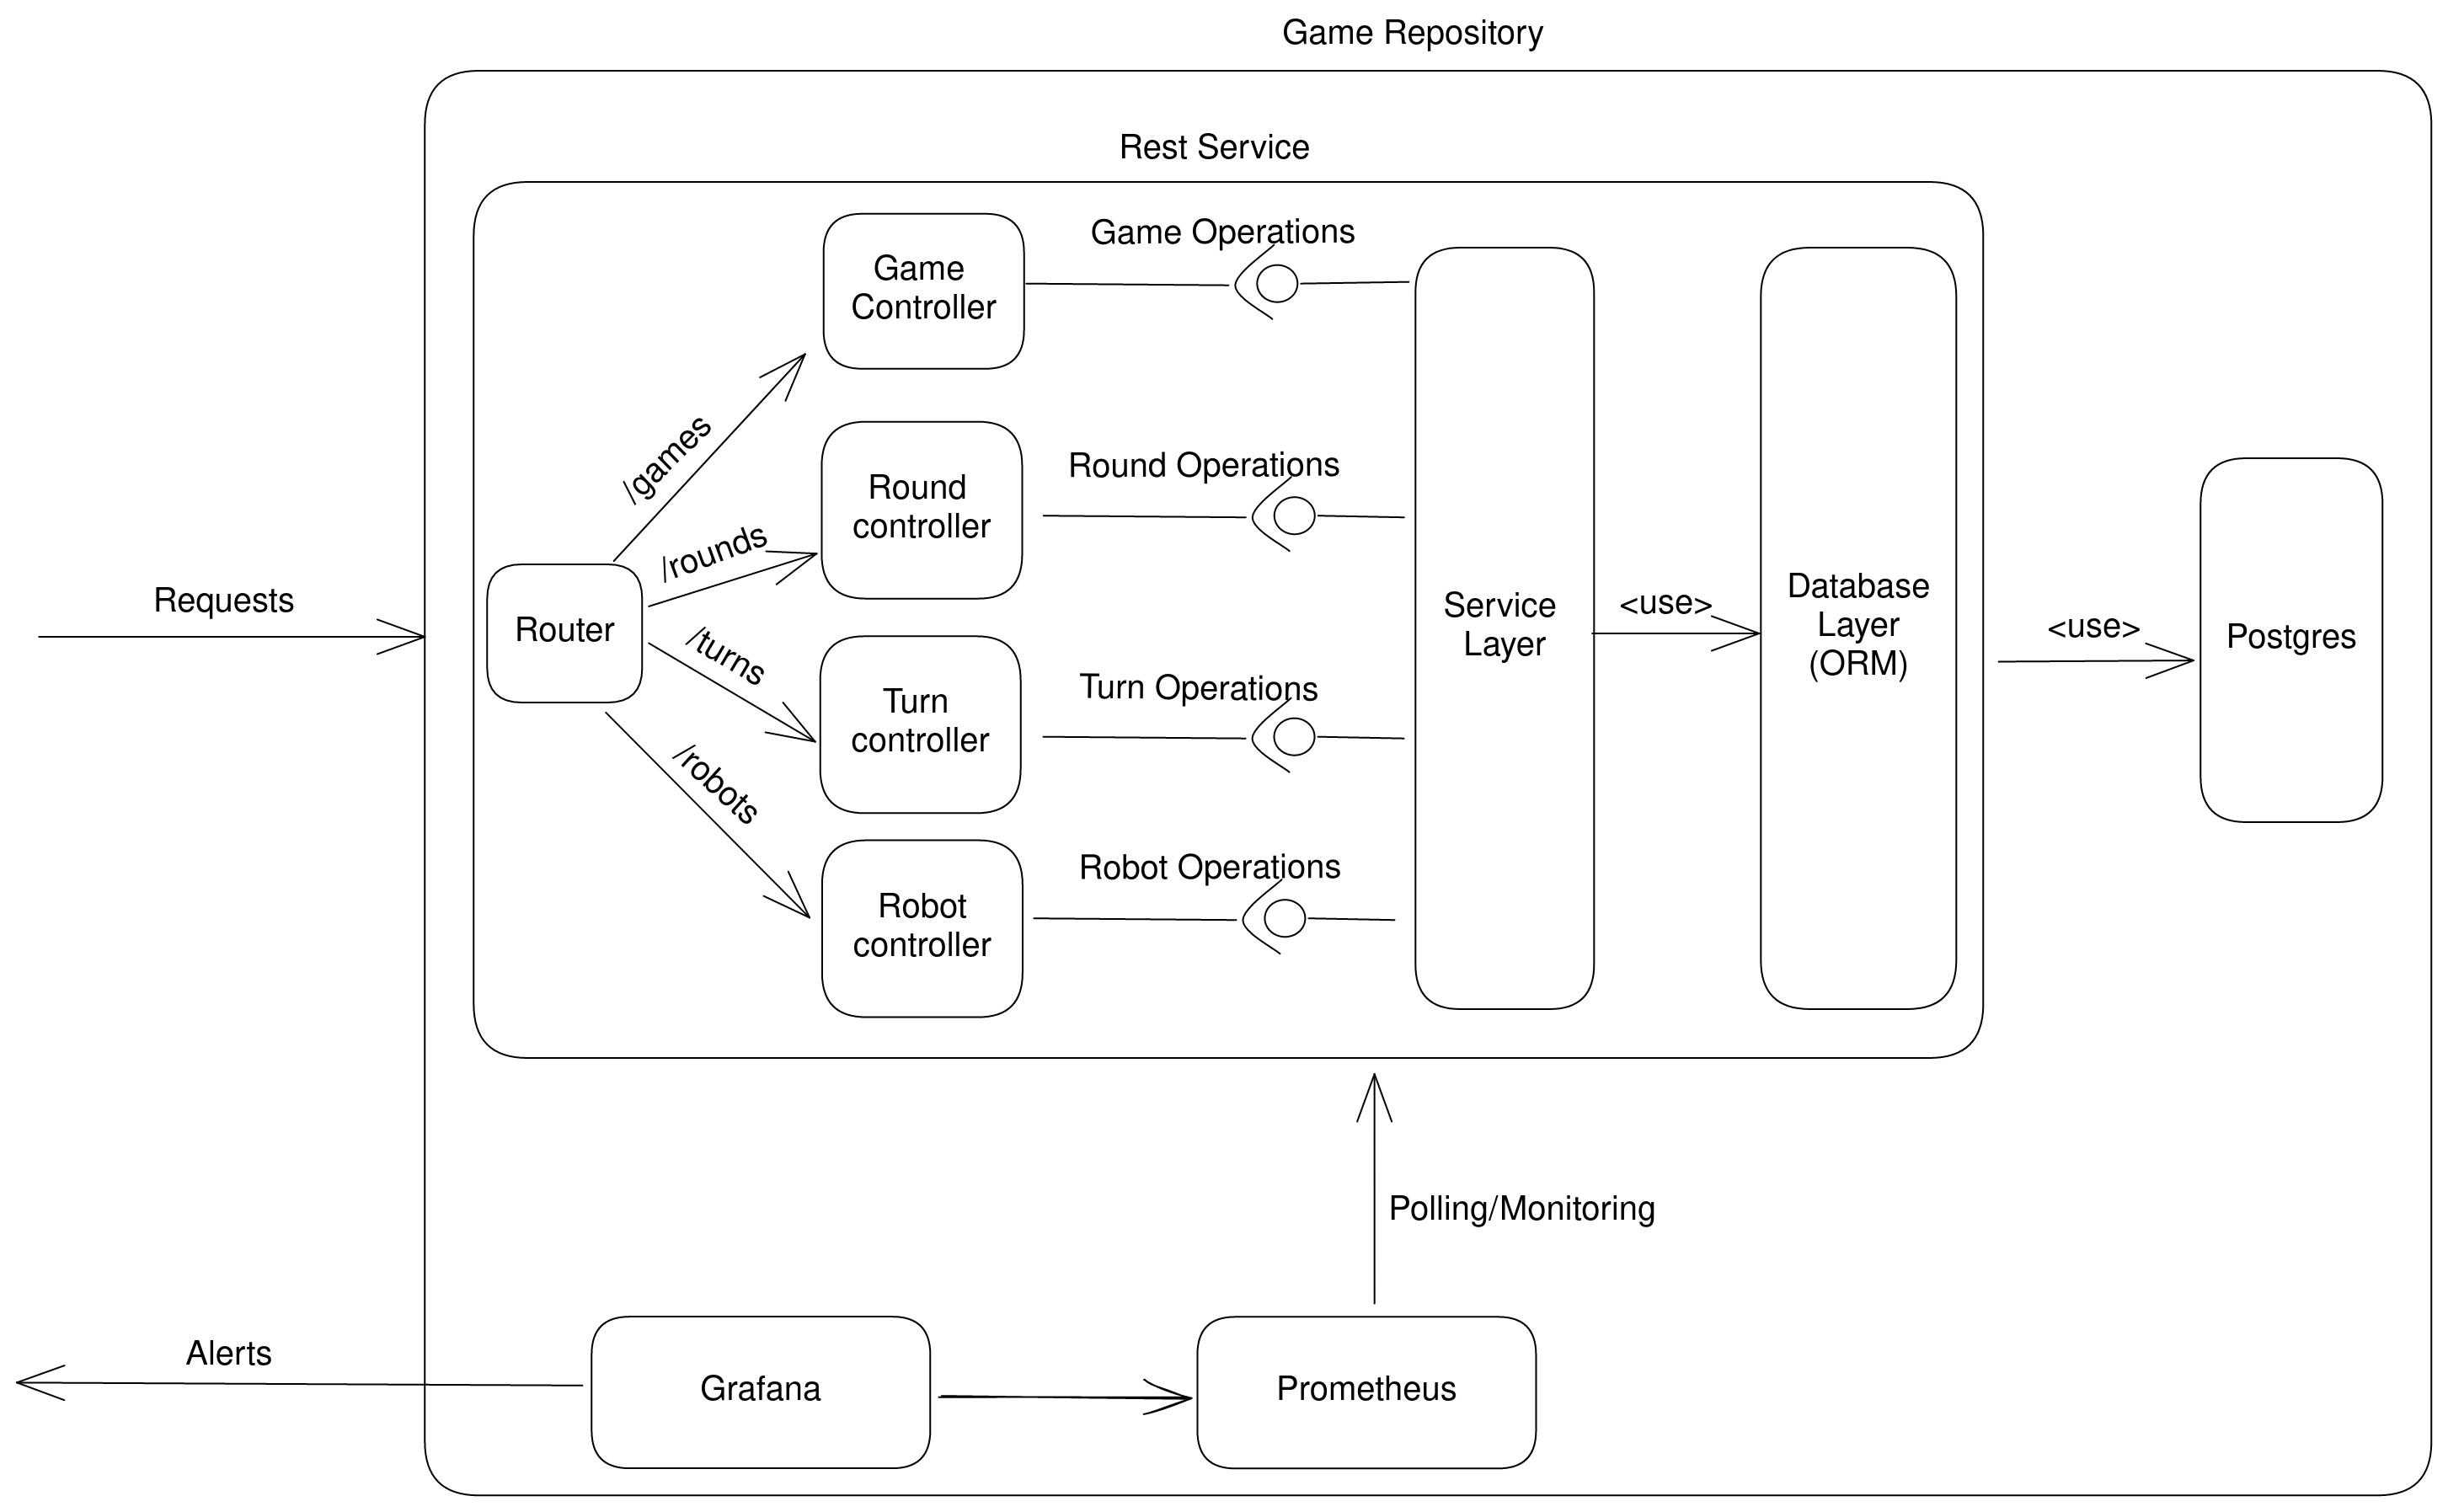
\includegraphics[width=\textwidth]{images/arch.png}
    \caption{Architettura della soluzione}
    \label{fig:arch}
\end{figure}

\subsection{Stato dell'applicazione}
Il componente è stato realizzato mediante un'architettura a servizi in cui sono coinvolte le seguenti entità:
\begin{itemize}
    \item Prometheus: componente che si occupa di raccogliere periodicamente le informazioni dai servizi configurati;
    \item Grafana: componente per la visualizzazione delle metriche con dashboard personalizzabili;
    \item Rest server: applicazione in Go che realizza un server HTTP e mette a disposizione delle API Rest con documentazione in OpenAPI;
    \item Postgres: database relazionale;
\end{itemize}

Tutti gli elementi elencati, ad eccezione del \textit{Rest Server} che è stato sviluppato dal team, sopra sono prodotti di terze parti \textit{Open Source}.
Il rest server è un'applicazione realizzata in Go configurabile con un file JSON specificato attraverso l'argomento \textit{config}. Attraverso un \textit{Makefile} è possibile:
\begin{itemize}
    \item compilare l'applicazione sia come \textit{binary standalone} che come immagine Docker;
    \item eseguire l'applicazione in un container;
    \item caricare l'immagine Docker su un server attraverso SSH;
\end{itemize}
\section{Attività svolte}
In questa sezione, saranno presentate le attività svolte.

\subsection{Raffinamento modello DB}

\subsubsection{Colonne "started\_at" e "closed\_at"}
Sono stati aggiunti gli attributi "started\_at" e "closed\_at" alle entità Game, Round e Turn allo scopo di registrare i momenti in cui uno di questi inizia o finisce.
Questo permetterà con più facilità al game engine di controllare lo stato del gioco, che prima di questa aggiunta poteva accedere solo alla data di creazione e modifica.

\subsubsection{Aggiunta entità "Robot"}
È stata creata una nuova entità "Robot", separata da quella "player", in seguito alla modifica architetturale e di funzionamento maturata durante le discussioni della seconda iterazione. Si è infatti realizzato che non sarebbe utile compilare e testare in ogni partita i risultati dei Robot, ma che basterebbe farlo solo all'atto della creazione del livello (test\_class) per poi memorizzare i punteggi e i file nel repository.
Per il robot \textit{Randoop} si è previsto inoltre di poter memorizzare più risultati, e di poterne recuperare uno casuale.
Gli attributi dell'entità Robot sono:
\begin{itemize}
    \item id: codice identificativo 
    \item id\_test\_class: il codice relativo alla classe da testare (livello)
    \item  scores: i punteggi relativi alla classe testata dal robot
    \item difficulty: livello di difficoltà del robot
    \item type: il tipo di robot (Evosuit o Randoop)
    \item created\_at: data di creazione
    \item updated\_at: data di modifica
\end{itemize}

È possibile osservare le modifiche apportate nella figura \cref{fig:er}. 

\subsection{Aggiunta API}
Sono state aggiunte le seguenti API:
\begin{itemize}
    \item Create Bulk Robots: crea dei risultati relativi a più robot per la classe specificata. Di seguito è mostrato il body della richiesta:
    \begin{lstlisting}[language=json,firstnumber=1]
    {
      "robots": [
        {
          "difficulty": "easy_v1",
          "type": "randoop",
          "scores": "some scores in some format",
          "testClassId": "a_test_class.java"
        }
      ]
    }
    \end{lstlisting}
    \item Get Robot by Filter: restituisce i punteggi relativi a un robot in base ai filtri \textit{test\_class\_id}, \textit{difficulty} e \textit{type}. 
    \item Delete Robot by Test Class: cancella i risultati dei Robot relativi a una classe di test specificata. 
\end{itemize}

Sono state inoltre aggiornate le seguenti API:
\begin{itemize}
    \item Get Games: aggiunta la possibilità di filtrare i risultati in base al nome del giocatore e ricevere una lista con tutte le sue partite.
    \item Create Turns: ora è possibile creare in massa i turni inviando la lista dei giocatori e il codice del round.
    Di seguito è mostrato il body della richiesta:
    \begin{lstlisting}[language=json,firstnumber=1]
    {
  "players": [
    "id1",
    "id2"
    ],
  "roundId": 1
    }
    \end{lstlisting}


\end{itemize}


\clearpage

\subsection{Implementazione Rate limiting}
Per proteggere l'API da attacchi DDoS è stato predisposto un sistema di \textit{rate limiting} che implementa l'algoritmo \textit{\textbf{Token Bucket}}. Uno schema dell'algoritmo è mostrato in \cref{fig:rate_limiting}.

Questo componente è configurabile con 3 parametri:
\begin{itemize}
    \item Requests per seconds: numero di richieste al secondo prima di ottenere un errore;
    \item Bursts: numero di token presenti nel bucket, quando sono esauriti il client viene messo in attesa;
    \item Enabled: quando è impostato a \textit{False} il \textit{rate limiting} viene disattivato;
\end{itemize}

Il rate limiting viene applicato per client: per fare questo è stato aggiunta una funzione alla catena di \textit{middleware} dei controller che si occupa di recuperare l'ip dell'\textit{host} originale nel caso in cui l'applicazione sia preceduta da \textit{gateway} e/o \textit{reverse proxy}. Infatti, un'applicazione posizionata alle spalle di un \textit{reverse proxy}, ha come indirizzo sorgente delle richieste \textit{HTTP} quello del \textit{proxy} che per convenzione (per non perdere l'informazione) spostano all'interno di header standard quali \textit{X-Forwarded-For}, \textit{X-Real-IP} o \textit{True-Client-IP}.

\begin{figure}[h]
    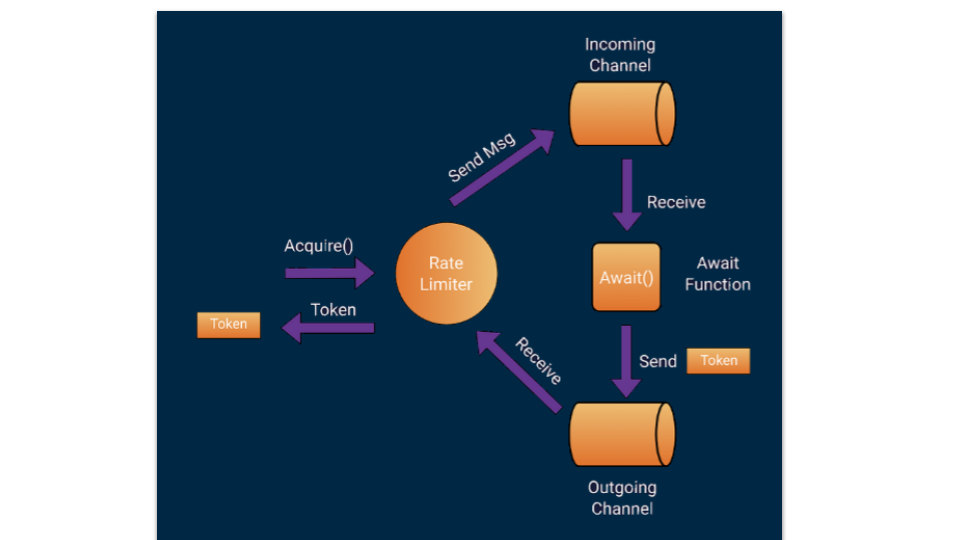
\includegraphics[width=\textwidth]{images/rate_limiting.png}
    \caption{Algoritmo token bucket}
    \label{fig:rate_limiting}
\end{figure}


\clearpage

\subsection{Implementazione CI/CD}
\subsubsection{Continous Integration}
Al momento l'applicazione esegue degli \textit{unit test} (che non prevedono l'utilizzo di un \textit{database}) quando vengono effettuate delle operazioni sul \textit{branch \textbf{master}} attraverso le \textit{Github Actions}. \\
In questa iterazione, è stata aggiunta la possibilità di eseguire dei test di integrazione con un database reale. In particolare, è stato aggiunto il \textit{target} \textit{test-integration} all'interno del \textit{Makefile} che esegue tutti i test nel sistema e calcola la copertura del codice. Il \textit{target} accetta in ingresso il flag \textit{CI} che permette di ottenere i seguenti comportamenti:
\begin{itemize}
    \item \textit{CI=1}: attraverso il parametro \textit{DB\_URI} viene specificato un'istanza già esistente per il database. L'operazione comporta la perdita di dati;
    \item CI non specificato: viene creata un'istanza usa e getta del database con Docker;
\end{itemize}

\subsubsection{Continous Deployment}
Come specificato nelle precedenti iterazioni, l'applicazione contiene una versione in esecuzione \hyperlink{qui}{https://sad.capass.org}. Con l'aggiunta dello script di \textit{Continous Deployment} (\cref{fig:cd}), attivato dalla creazione di una nuova \textit{release}, si effettuano le seguenti azioni:
\begin{itemize}
    \item Build con Docker: viene creata un'immagine Docker che viene salvata sul \textit{repository} pubblico \textit{capas/game-repository};
    \item Deploy della versione live: con SSH, viene aggiornata l'applicazione sul server;
    \item Pubblicazione di \textit{artifact}: con riferimento alla matrice architettura/sistema operativo in \cref{tab:comp_matrix}, per ciascuna cella supportata viene creato un archivio contenente: l'eseguibile, file di licenza, README.md, specifica OpenAPI e una collection Postman per gli facilitare l'integrazione con gli altri componenti;
\end{itemize}

\begin{table}[h]
    \centering
    \begin{tabular}{|l|l|l|l|l|}
        \hline
         Arch/OS & Linux & Windows & Darwin \\
        \hline
        \hline
         i386 & x & x &  \\
         amd64 & x & x & x \\
         arm64 & x & & x  \\
        \hline
    \end{tabular}
    \caption{Matrice di compatibilità supportata}
    \label{tab:comp_matrix}
\end{table}

\begin{figure}
    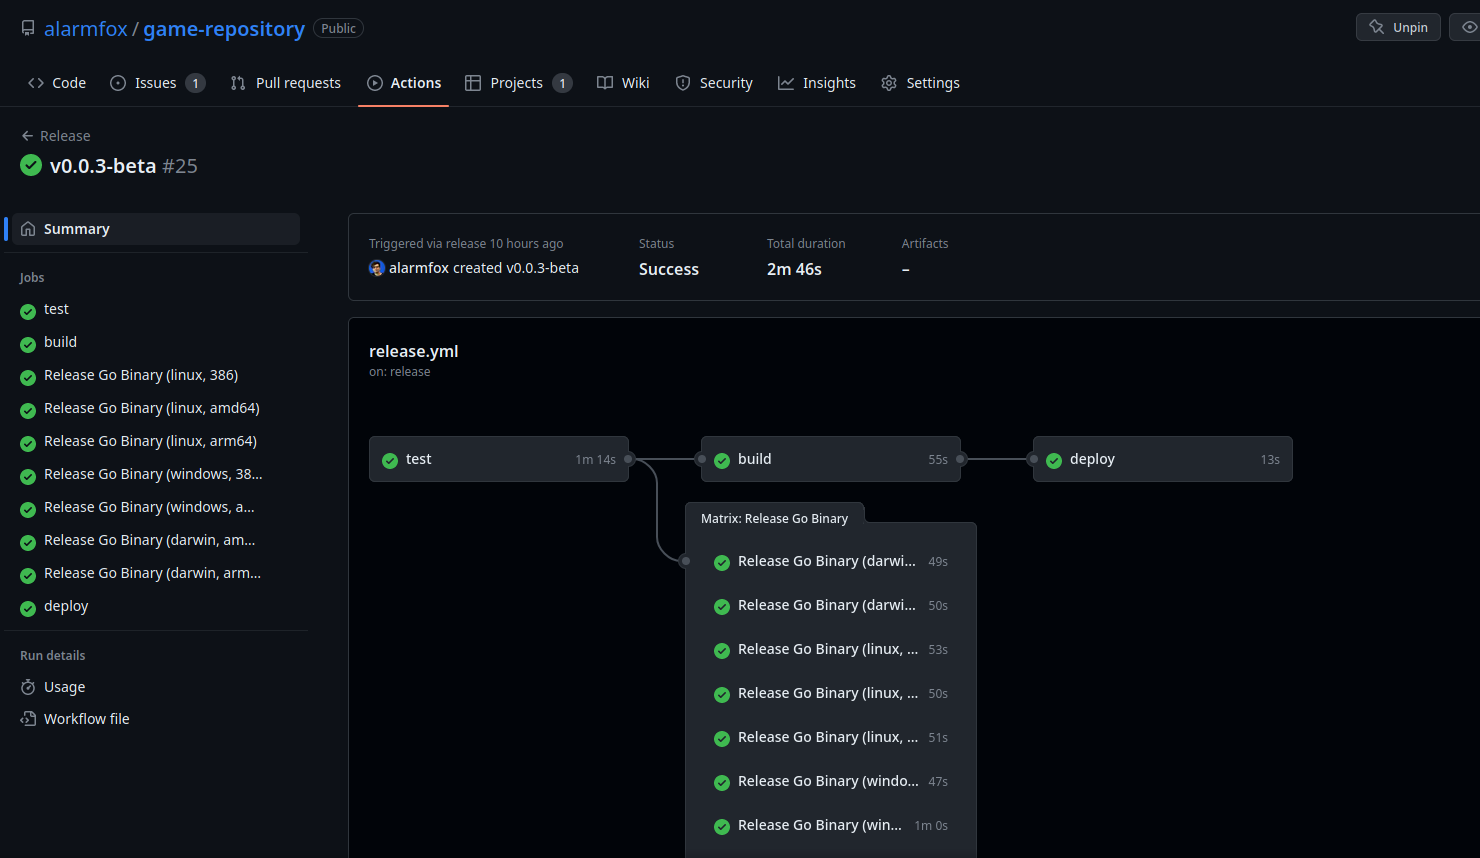
\includegraphics[width=\textwidth]{images/cd.png}
    \caption{Esecuzione dello script CD per la release 0.0.3-beta}
    \label{fig:cd}
\end{figure}

\paragraph{Documentazione self-building}
Insieme al Continous Ceployment dell'applicazione è stata creata con l'utilizzo di \textit{MkDocs} una documentazione in cui si spiega tecnicamente la struttura del progetto, le modalità di installazione e configurazione (\cref{fig:docs}). Analogamente, all CI/CD è stato creato uno script che utilizza Github Actions per effettuare un aggiornamento della documentazione laddove ci sia un aggiornamento dei file nel \textit{path docs/}. In particolare, l'applicazione viene ospitata grazie a Github Pages che consente di usufruire di un server http che effettua il \textit{serving} statico dei file. Attualmente la documentazione si trova a questo  \hyperlink{link}{https://alarmfox.github.io/game-repository}

\begin{figure}[h]
    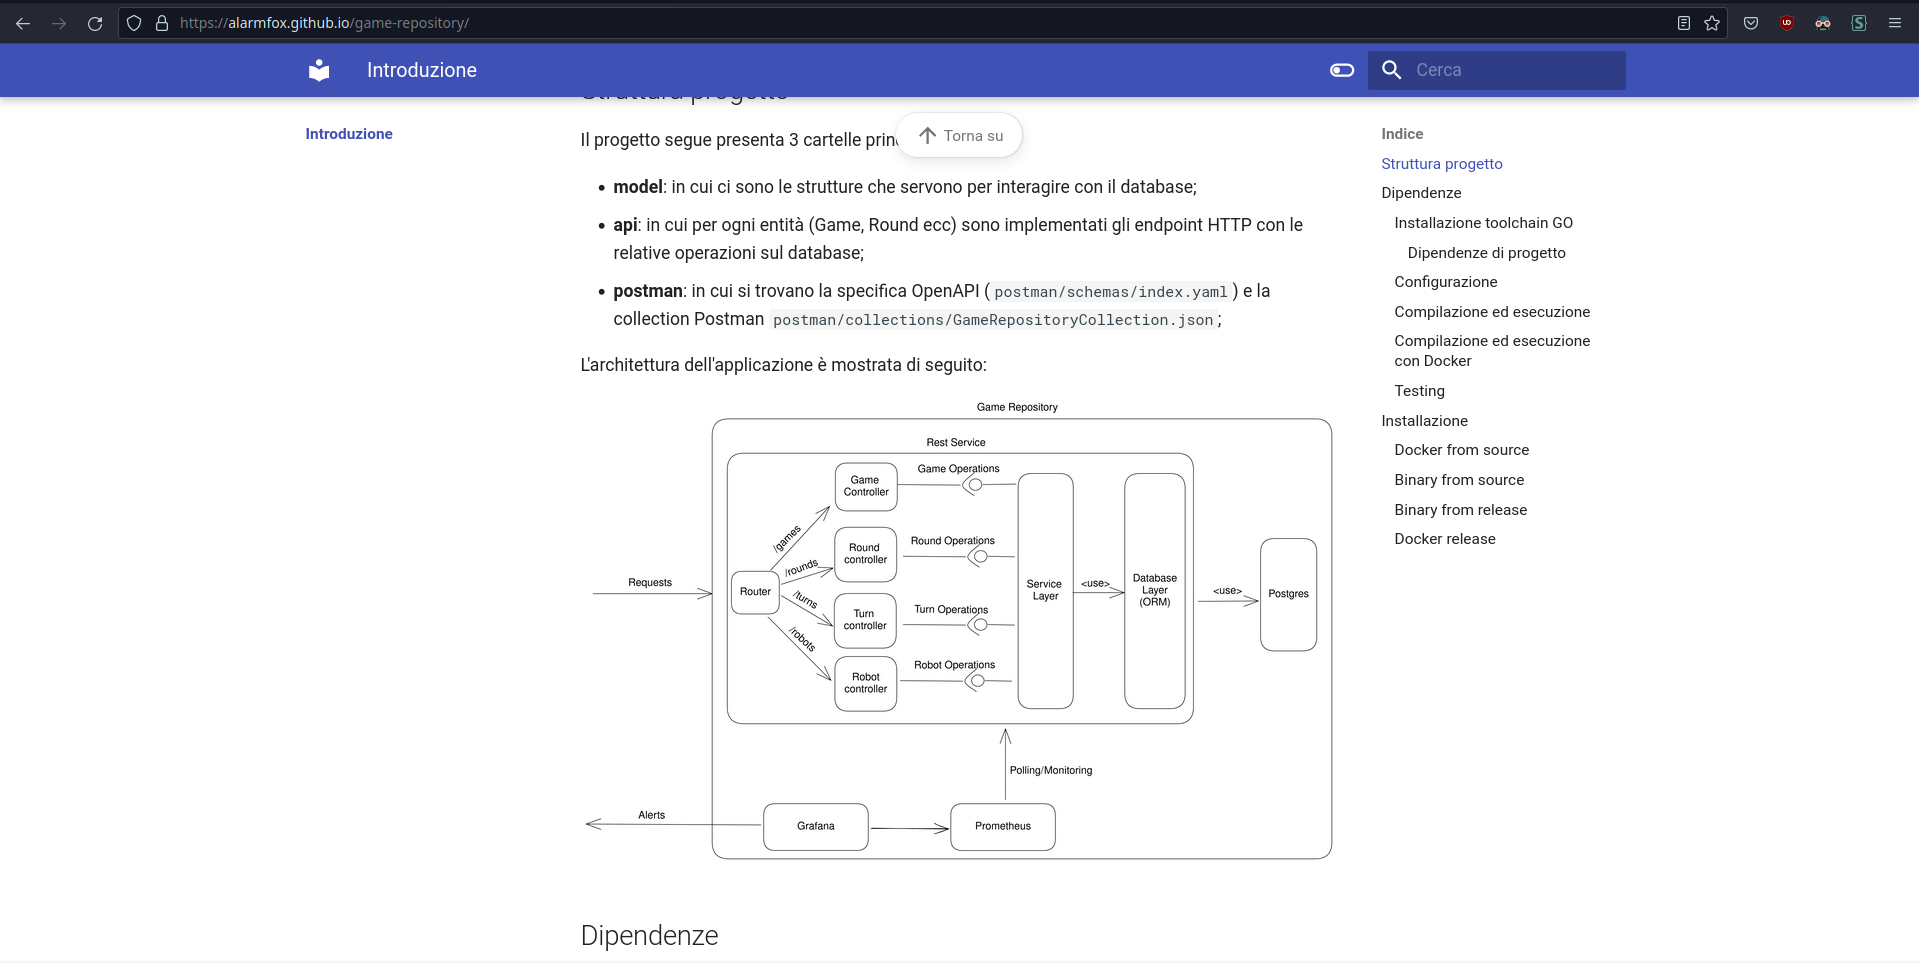
\includegraphics[width=\textwidth]{images/docs.png}
    \caption{Documentazione di progetto}
    \label{fig:docs}
\end{figure}

\clearpage

\printbibliography

\end{document}